\chapter{Trabajo relacionado}\label{chap:trabajo_relacionado}

Dentro de este capitulo se presenta un resumen de diseños de redes en chip especificas para dispositivos reconfigurables. Cada trabajo aborda el tema de optimización de diseño tomando ventaja de alguna de las características particulares para dispositivos FPGA.

\section{Redes en-chip en FPGA}\label{sec:redes_en_chip_en_fpga}

La universidad Brigham Young en conjunto con la corporación Ricon Research desarrollaron una arquitectura exclusiva para dispositivos reconfigurables de nombre \smallcaps{PNoC}\cite{chapter3:1515721, chapter3:1626510}. La arquitectura se caracteriza por el uso del concepto de isla de procesamiento, cada isla está formada por un conjunto de bloques propietarios funcionales y un router para la interconexión de todos ellos. El router de PNoC utiliza conmutación de circuitos para crear enlaces de comunicación entre sus miembros, además, utiliza tablas de encaminamiento para todos los cálculos de ruta. La figura \ref{fig:ch3_pnoc} muestra la organización de una red PNoC.

El uso de tablas de ruteo permite la implementación de un sistema sencillo de transmisión masiva (broadcast) para todos los miembros de la red. En cuanto a escalabilidad, PNoC permite el uso de un puerto de salida para la comunicación con otras islas de procesamiento, permitiendo la interconexión de múltiples islas. La interacción entre unidades funcionales y estructura de interconexión se lleva a cabo por medio de estructuras FIFO, permitiendo el uso de diferentes frecuencias de operación entre miembros de la red.

\begin{figure}
	\begin{center}
		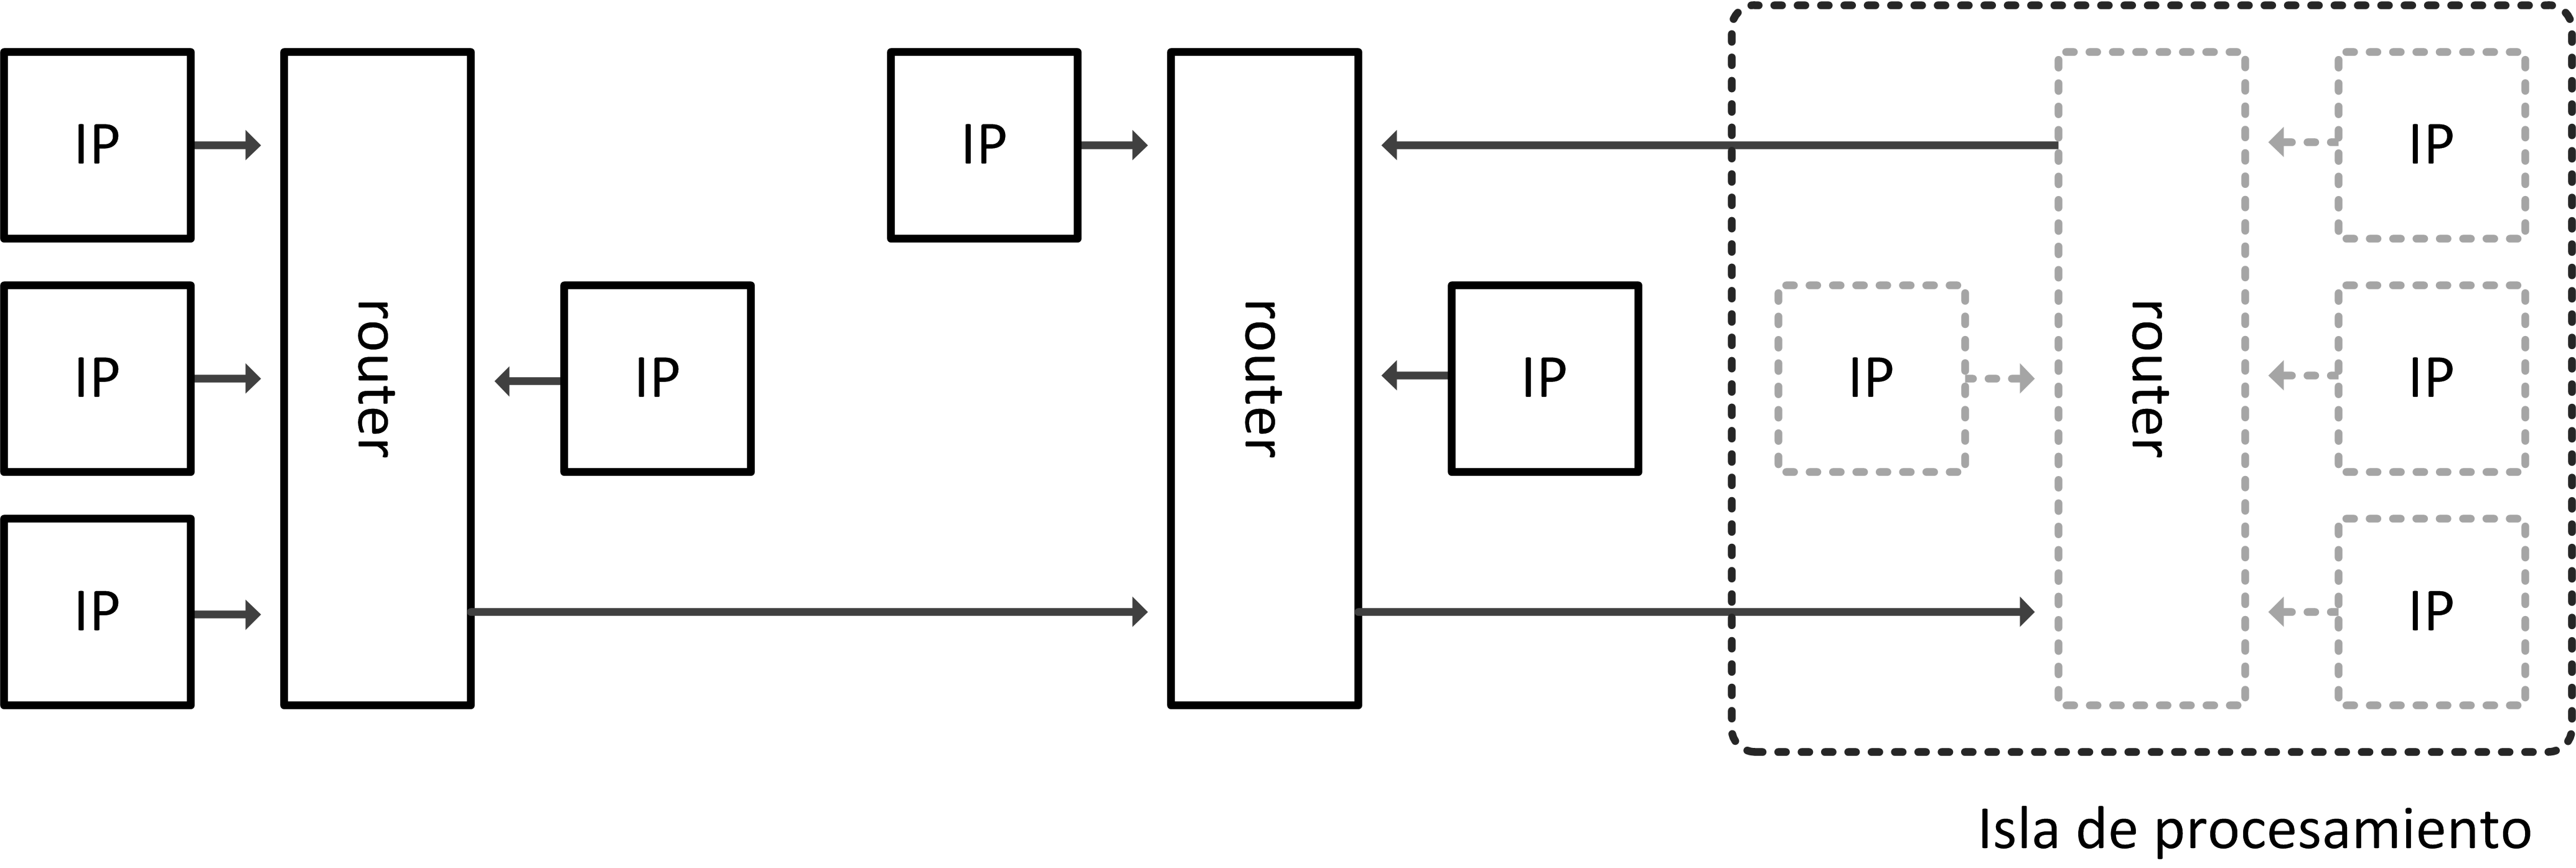
\includegraphics[scale=0.6]{figures/ch3_pnoc.png}
	\end{center}
	\caption
		{	
			Diagrama a bloques de red PNoC. La comunicación entre islas permite escalar el número de unidades funcionales del sistema. Además, el uso de múltiples isla permite la distribución de la demanda de recursos en diferentes áreas del sistema.
		}
	\label{fig:ch3_pnoc}
\end{figure}

Jovanovic \textit{et al.} presenta la arquitectura denominada \smallcaps{CuNoC}\cite{chapter3:4380761}. El uso de una topología tipo malla y una estrategia de conmutación de paquetes define el comportamiento para esta red. La cualidad principal de este trabajo es el uso de routers denominados \textit{Communication Unit}. Este último busca reducir el número de recursos necesarios para su implementación, en específico los requerimientos de elementos de memoria, eliminando de cada router cualquier forma de medio de almacenamiento temporal en sus puertos de salida. En lugar de unidades de almacenamiento distribuidas en cada puerto de salida, se ofrece una unidad de almacenamiento centralizada para todos los paquetes en transito a través del encaminador.

Todos los paquetes entrantes al encaminador de la red CuNoC deben de ser almacenados en el espacio de memoria común antes de poder ser propagados a una salida del router. El proceso de liberación de un paquete a la red requiere de 2 ciclos de reloj adicionales a la latencia generada por el tráfico de paquetes dentro del encaminador. La figura \ref{fig:ch3_cunoc} muestra el esquema de almacenamiento propuesto por CuNoC. Para los cálculos de trayectoria a través de la red se utiliza una versión modificada del algoritmo \textit{XY}, la cual permite la inclusión del tráfico presente en los vecinos de cada nodo de la red para la toma de decisión de la ruta a seguir.

\begin{figure}
	\begin{center}
		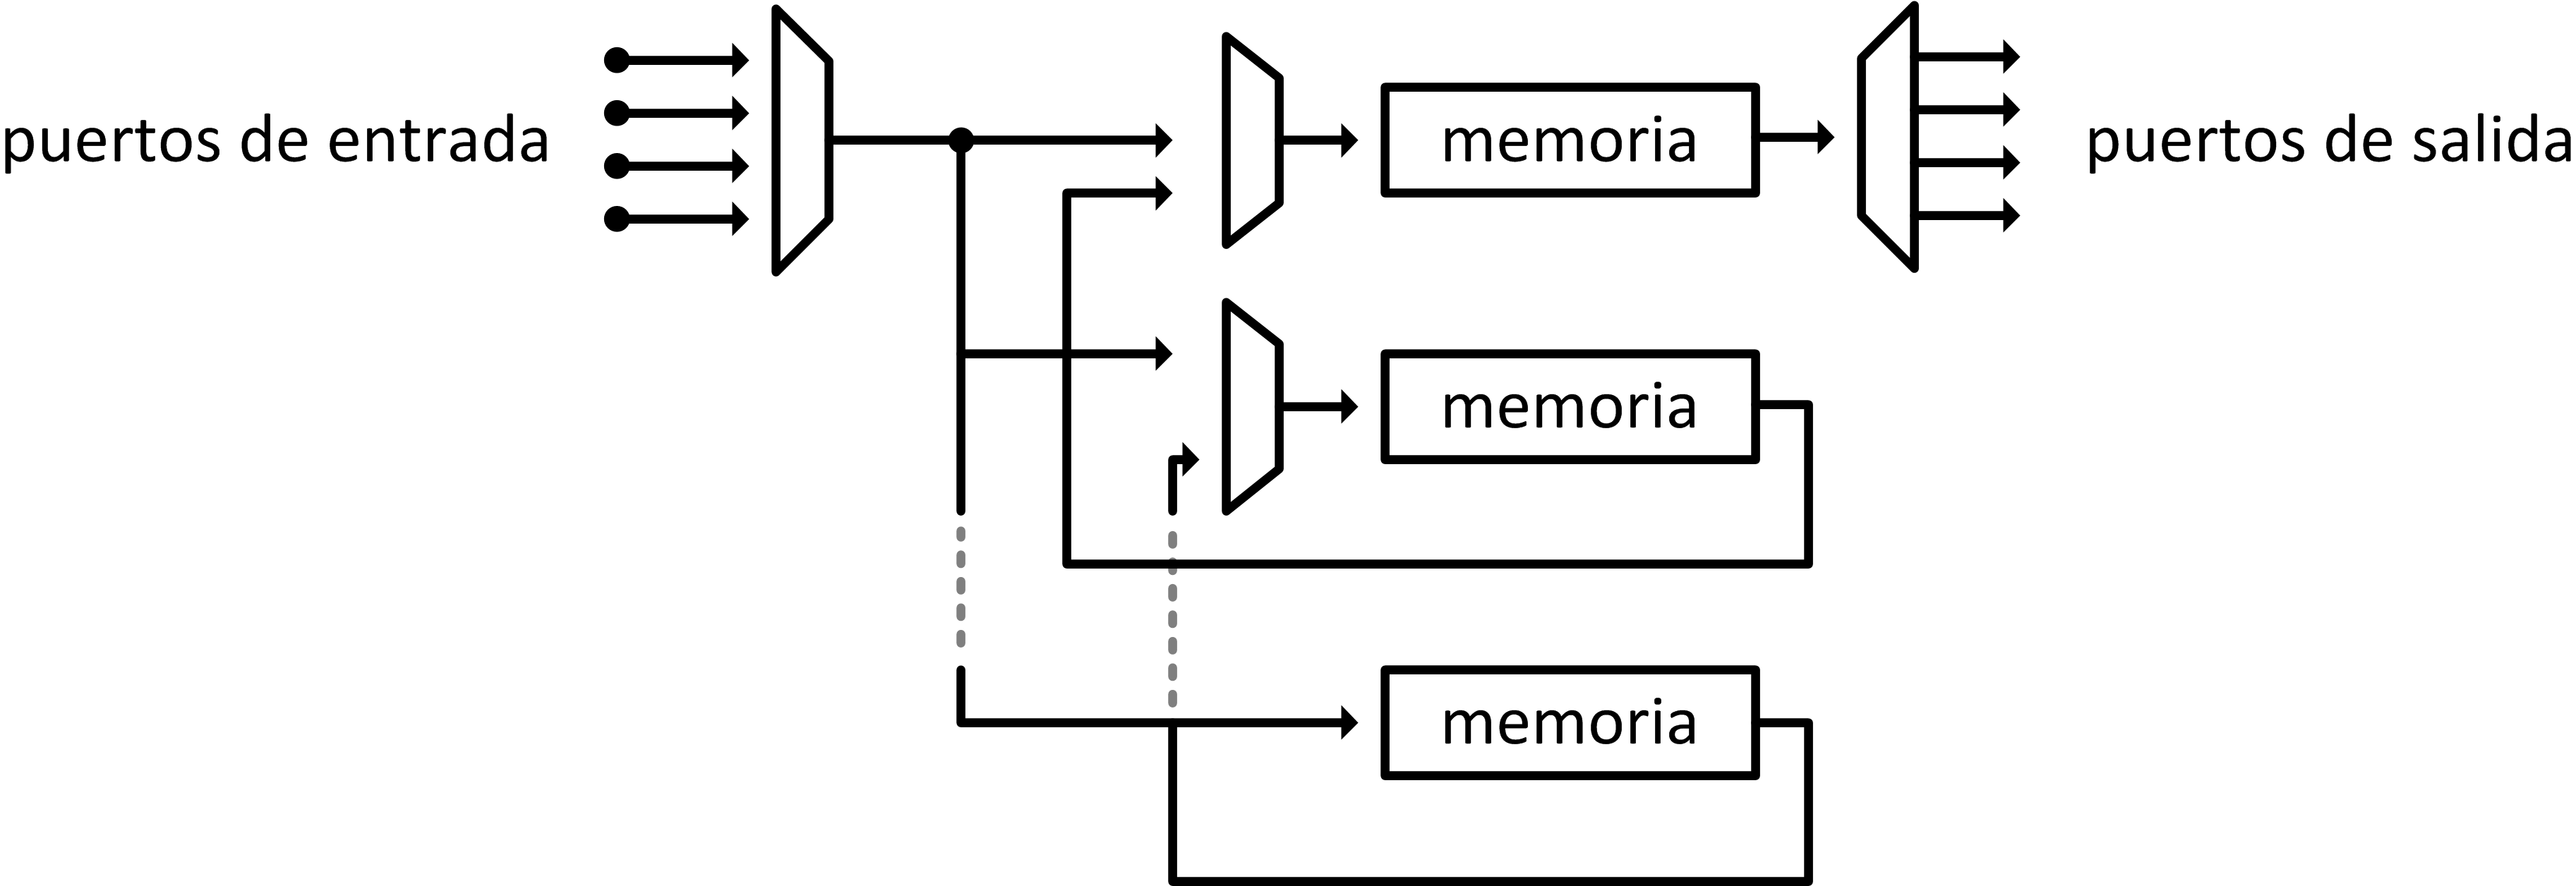
\includegraphics[scale=0.6]{figures/ch3_cunoc.png}
	\end{center}
	\caption
		{	
			La estructura central de almacenamiento para los paquetes entrantes a un router CuNoC representa una disminución en los recursos necesarios para su implementación, sin embargo, crea un cuello de botella para el envío rápido de información hacia su siguiente salto en la red.
		}
	\label{fig:ch3_cunoc}
\end{figure}

\smallcaps{Quark}\cite{chapter3:5076186, chapter3:4724383, chapter3:5161210, chapter3:4724416} es una red en-chip que propone una topología \textit{Spidergon}\cite{chapter3:1411133, chapter3:4221002} modificada. En una topología Spidergon tradicional cada nodo de la red presenta canales de comunicación con sus vecinos izquierdo, derecho y diagonalmente opuesto. En particular, el canal diagonal presenta cargas de trabajo mayores que sus contrapartes laterales debido a ser el único camino para alcanzar los nodos opuesto de la red. Para reducir la carga en este enlace \textit{Quark} propone el anexo de un nuevo canal diagonal para incrementar el ancho de banda disponible.

El algoritmo de encaminamiento propuesto para \textit{Quark} divide a los nodos miembro de la red en 4 cuadrantes, si el destino de una transferencia se encuentra en los cuadrantes vecinos al nodo, la red utilizará de manera constante los canales izquierdo o derecho para enviar el paquete. En caso que el destino se encuentre en los cuadrantes opuestos al nodo origen, la red utiliza el canal diagonal. El algoritmo mencionado anteriormente es determinístico, por lo que la red siempre utiliza las misma ruta para la transferencia de paquetes entre dos nodos.

Moraes \textit{et al.}\cite{chapter3:Moraes200469} presenta la arquitectura \smallcaps{Hermes}. La arquitectura se caracteriza por una topología tipo malla irregular, ya que existen dos modelos de router. Los nodos al centro de la red presentan 5 canales de comunicación mientras que los nodos a la periferia sólo ofrecen 4 puntos de interconexión. \textit{HERMES} se caracteriza por la reducción del consumo de recursos mediante el uso de una sola unidad de cálculo de ruta para todos los puertos del router. El proceso de arbitraje, cálculo de ruta y reenvío de paquete toma a un nodo de \textit{HERMES} dos ciclos de reloj, sin embargo, solo puede atender una sola petición a la vez. El uso de multiplexado en tiempo de la unidad de cálculo de ruta impone una fuerte restricción en rendimiento para esta red.

Janarthanan \textit{et al.} presentan la arquitectura \smallcaps{MoCReS}\cite{chapter3:4208959}, una red en-chip específica para dispositivos reconfigurables. El diseño sobresale por su propuesta de integración de canales virtuales, de longitud variable,  mediante el uso de bloques rígidos de memoria BRAM. El uso de bloques propietarios de memoria limitan la implementación del sistema a dispositivos fabricados por Xilinx. Los autores del trabajo resalta la disminución en el consumo de elementos reconfigurables al utilizar bloques BRAM como medio de almacenamiento temporal. \textit{MoCReS} utiliza el algoritmo determinístico \textit{XY} para la planificación de rutas de transmisión de paquetes. La arquitectura de este trabajo deja pasar la oportunidad del uso de algoritmos de encaminamiento adaptativos aun cuando se cuenta con canales virtuales.

\smallcaps{SoCWire}\cite{chapter3:584254, chapter3:5546220}, una red en-chip diseñada para dispositivos reconfigurables en aplicaciones espaciales, destaca por su compatibilidad con el protocolo SpaceWire\cite{chapter3:4584258, chapter3:1547397, chapter3:1655950, chapter3:4526504, chapter3:5197252} utilizado por la agencia espacial Europea. Una red SoCWire está formada por routers capaces de ofrecer servicio de comunicación a un máximo de 32 unidades funcionales. Otro punto destacable de este desarrollo es la habilidad de tomar ventaja de la capacidad de reconfiguración parcial\cite{chapter3:PR:Xilinx} de los dispositivos FPGA para permitir el intercambio de unidades funcionales del sistema sin perturbar su operación.

Los puertos del router con compatibilidad para el protocolo SoCWire descomponen los mensajes a un formato de trama intermedio que el router utiliza para la entrega de mensajes entre unidades funcionales. De igual forma, una trama de datos que abandona el encaminador a través de un puerto con compatibilidad SoCWire, es transformada del formato intermedio del router a un mensaje del protocolo anteriormente mencionado. Los encaminadores ofrecen servicios de calidad de servicio como detección y corrección de errores durante la transmisión de mensajes.

Zeferino \textit{et al.} proponen la arquitectura parametrizable SoCIN\cite{chapter3:1232824}. Este trabajo propone el diseño de un encaminador parametrizado capaz de adecuarse para su implementación en redes con topologías tipo torus y malla. Una característica destacable es el cálculo de ruta procesado en las interfaces de red de cada nodo, de manera que la lógica necesaria para implementar los encaminadores se simplifica, al solo operar como decodificadores y retransmisores de información. La técnica de conmutación de paquetes es utilizada para la administración de recursos en los routers de la red y se utiliza la técnica \textit{wormhole} para el control de flujo de información.

Vale la pena resaltar que esta red utiliza un modelo maestro - esclavo para efectuar las transferencias de información entre nodos. Un nodo maestro debe de iniciar una transacción para comenzar el envío de mensajes, por su parte, el nodo esclavo se limita a la recepcion de informacion.

\smallcaps{RoC}\cite{chapter3:4511160, chapter3:4016946} es una red basada en una topología tipo anillo redundante. Esta arquitectura presenta un mecanismo minimalista para el manejo de paquetes a través de la red: cada paquete en tránsito es capturado por los encaminadores en su trayecto. Dentro del encaminador, se analiza la dirección destino del paquete, en caso de estar dirigido al nodo actual el encaminador retira el paquete de la red y lo transfiere a la unidad funcional, en caso contrario, el router propaga el paquete al siguiente encaminador. La interfaz de red de \textit{RoC} se encuentra fuertemente integrada al router, al grado de que resulta imposible distinguir actividades exclusivas de la interfaz. 

La interacción de encaminador con unidad funcional se lleva a cabo mediante una estructura de almacenamiento FIFO, la unidad funcional escribe datos al FIFO de router, el cual a su vez reserva el uso de un anillo para la inyección del nuevo paquete. En caso que todos los anillos se encuentren ocupados, el router almacena de manera temporal el paquete y espera por disponibilidad de canales de comunicación.

A. Ahmadinia \textit{et al.} proponen la arquitectura \smallcaps{RMBoC}\cite{chapter3:1509437, chapter3:1511976}, la cual consiste en un sistema híbrido entre red en-chip y una estructura de medio compartido. Los routers en una red \textit{RMBoC} se denominan unidad de punto de cruce con elemento de procesamiento, y prestan servicio de manera exclusiva a una unidad funcional. Cada unidad de punto de cruce tiene acceso a canales de comunicación con el vecino a la izquierda y derecha del nodo. El conjunto de todos los nodos de la red forma un medio compartido segmentado\cite{chapter3:Romine:1992:DSM:143487}, donde cada router es responsable de recibir peticiones y bloquear recursos para la formación de un enlace entre dos nodos. \textit{RMBoC} puede analizarse como una red en-chip unidimensional con conmutación de circuitos. La figura \ref{fig:ch3_rmboc} muestra un ensamble típico \textit{RMBoC}.

El manejo de contingencias durante una transmisión de \textit{RMBoC} consiste en el envío de una señal de bloqueo al nodo transmisor, el cual, al recibir esta señal procederá a la liberación de todos los canales de comunicación reservados y esperará un tiempo de guarda para reintentar la transacción deseada.

\begin{figure}
	\begin{center}
		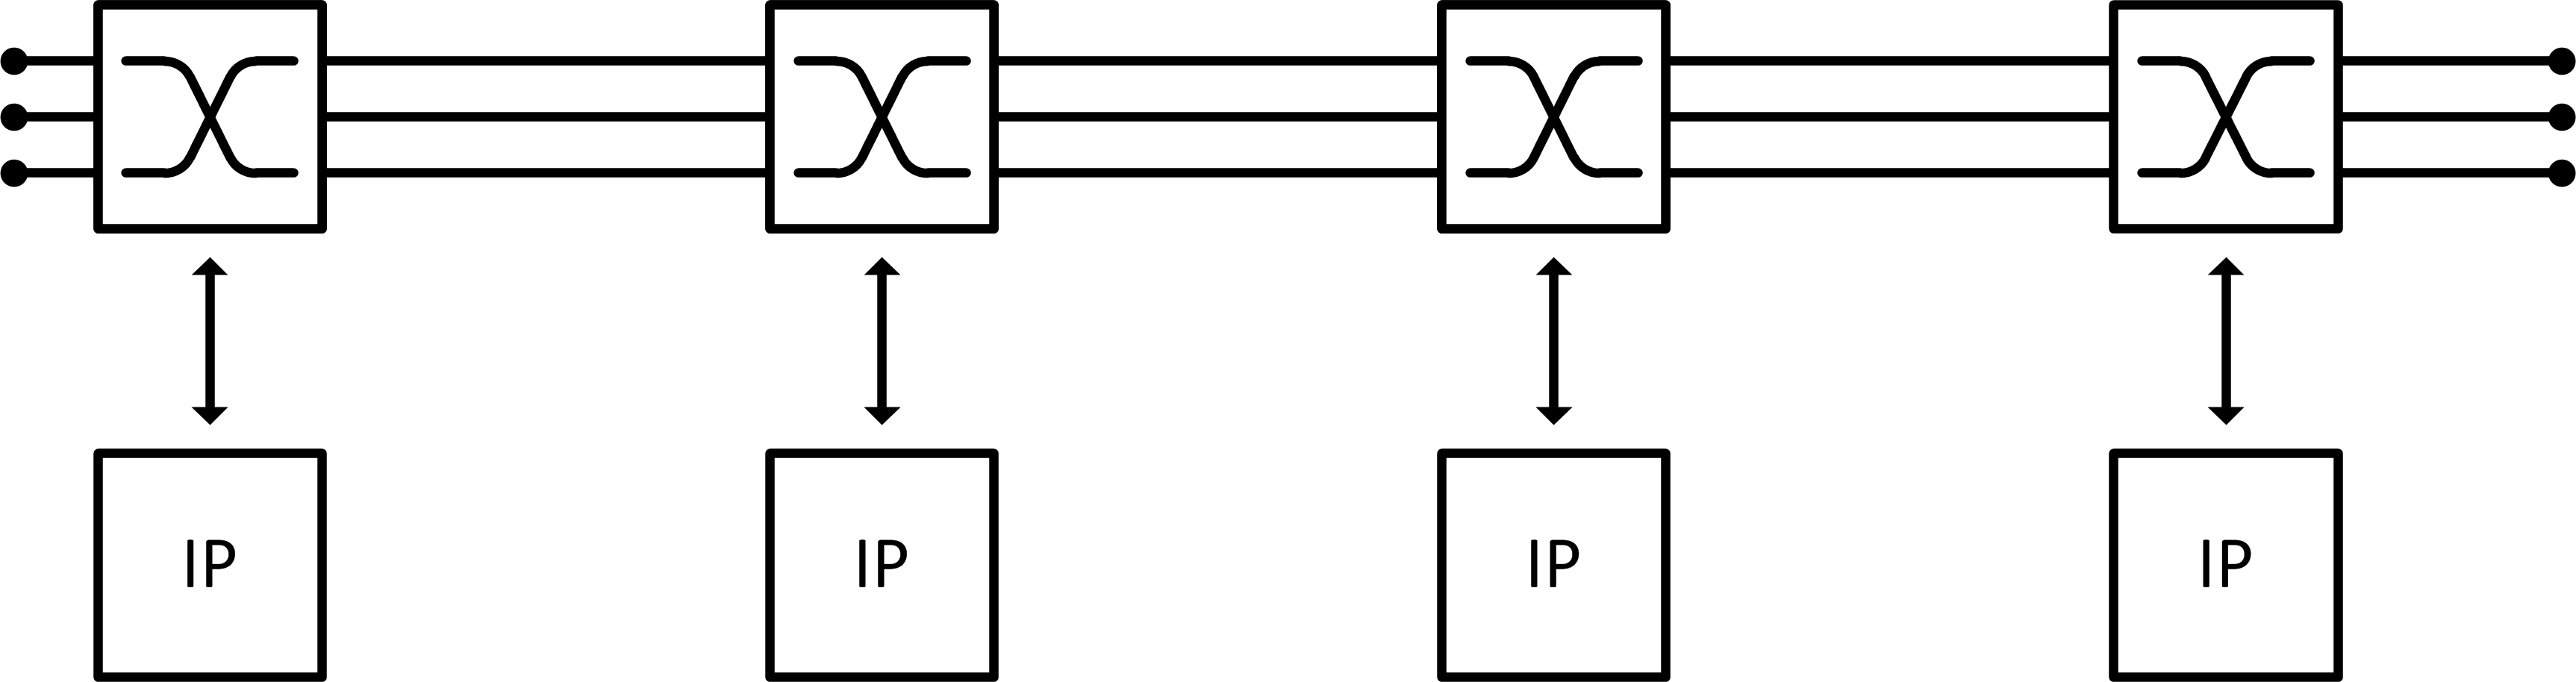
\includegraphics[scale=0.6]{figures/ch3_rmboc.png}
	\end{center}
	\caption
		{	
			RMBoC Utiliza un híbrido entre un medio compartido y una conmutación de circuitos, para incrementar su rendimiento requiere de un aumento delineas de interconexión que pueden resultar costosas para sistemas en-chip.
		}
	\label{fig:ch3_rmboc}
\end{figure}

\smallcaps{DyNoC}\cite{chapter3:1515715} es una red en-chip con topología tipo malla que sobresale por el uso del algoritmo de encaminamiento denominado S-XY\cite{chapter3:1511976}, el cual tiene la capacidad de cambiar de dirección en caso de encontrar una ruta con bloqueo y regresar al camino original una vez sorteado el obstáculo en su ruta original. En su trabajo Bobda \textit{et al.} proponen una red \textit{DyNoC} saturada con encaminadores, de esta manera proveen de un mayor número de rutas alternas para el desvios de transmisiones en caso de bloqueo.

Pionteck \textit{et al.}\cite{chapter3:4100970} desarrollaron la arquitectura de red en-chip denominada \smallcaps{CoNoChi}, su principal característica es el estar diseñada para ejecutar operaciones de reconfiguración dinámica a nivel de unidades funcionales y encaminadores. El mecanismo de manejo de ruta de esta red está basado en tablas, cada tabla se encuentra alojada en un bloque de memoria rígido, el cual puede agregar o modificar entradas en base a comandos de red. Esta capacidad de edición de las tablas de encaminamiento permite a \textit{CoNoChi} el agregar nuevas unidades funcionales al sistema, además de permitir la salida de otras sin crear caminos inválidos para la transferencia de paquetes. La tabla \ref{tap:ch4_comparativa} presenta un resumen de los trabajos expuestos.


\begin{sidewaystable}

\centering
\begin{tabular}{@{}ccccccccc@{}}
\toprule
\rowcolor[HTML]{656565} 
{\color[HTML]{FFFFFF} \textbf{NoC}} & {\color[HTML]{FFFFFF} \textbf{Topología}}                                         & {\color[HTML]{FFFFFF} \textbf{\begin{tabular}[c]{@{}c@{}}Relacion\\ con EP\end{tabular}}} & {\color[HTML]{FFFFFF} \textbf{\begin{tabular}[c]{@{}c@{}}Algoritmo de\\ calculo de\\ ruta\end{tabular}}} & {\color[HTML]{FFFFFF} \textbf{\begin{tabular}[c]{@{}c@{}}Tipo de\\ conmutacion\end{tabular}}} & {\color[HTML]{FFFFFF} \textbf{\begin{tabular}[c]{@{}c@{}}frecuencia\\ de\\ operación\end{tabular}}} & {\color[HTML]{FFFFFF} \textbf{\begin{tabular}[c]{@{}c@{}}Ocupación\\ (Slices)\end{tabular}}} & {\color[HTML]{FFFFFF} \textbf{\begin{tabular}[c]{@{}c@{}}Ancho de\\ palabra de\\ datos (bits)\end{tabular}}} & {\color[HTML]{FFFFFF} \textbf{\begin{tabular}[c]{@{}c@{}}Ancho\\ de banda\end{tabular}}} \\ \midrule
PnoC                                & crossbar                                                                          & \begin{tabular}[c]{@{}c@{}}red\\ indirecta\end{tabular}                                   & \begin{tabular}[c]{@{}c@{}}tablas de \\ ruteo\end{tabular}                                               & \begin{tabular}[c]{@{}c@{}}conmutación\\ de circuitos\end{tabular}                            & 126 MHz                                                                                             & 1223                                                                                         & 8                                                                                                            & NP                                                                                       \\
\rowcolor[HTML]{EFEFEF} 
CuNoC                               & malla                                                                             & \begin{tabular}[c]{@{}c@{}}red\\ indirecta\end{tabular}                                   & DOR XY                                                                                                   & \begin{tabular}[c]{@{}c@{}}Store \&\\ forward\end{tabular}                                    & 241 MHz                                                                                             & 128                                                                                          & 32                                                                                                           & NP                                                                                       \\
Quark                               & spidergon                                                                         & \begin{tabular}[c]{@{}c@{}}red\\ directa\end{tabular}                                     & \begin{tabular}[c]{@{}c@{}}calculo de \\ cuadrante\end{tabular}                                          & wormhole                                                                                      & NP                                                                                                  & 1453                                                                                         & 32                                                                                                           & NP                                                                                       \\
\rowcolor[HTML]{EFEFEF} 
Hermes                              & malla                                                                             & \begin{tabular}[c]{@{}c@{}}red\\ directa\end{tabular}                                     & DOR XY                                                                                                   & wormhole                                                                                      & 25 MHz                                                                                              & 316                                                                                          & 10                                                                                                           & 500 Mbps                                                                                 \\
MoCReS                              & malla                                                                             & \begin{tabular}[c]{@{}c@{}}red\\ directa\end{tabular}                                     & DOR XY                                                                                                   & \begin{tabular}[c]{@{}c@{}}virtual\\ cut-through\end{tabular}                                 & 357 MHz                                                                                             & 282                                                                                          & 8                                                                                                            & 2.85 Gbps                                                                                \\
\rowcolor[HTML]{EFEFEF} 
SoCWire                             & múltiple                                                                          & \begin{tabular}[c]{@{}c@{}}red\\ directa\end{tabular}                                     & \begin{tabular}[c]{@{}c@{}}XY\\ modificado\end{tabular}                                                  & wormhole                                                                                      & 180 MHz                                                                                             & 1270                                                                                         & 32                                                                                                           & 2800 Mbps                                                                                \\
SoCIN                               & malla                                                                             & \begin{tabular}[c]{@{}c@{}}red\\ directa\end{tabular}                                     & DOR XY                                                                                                   & wormhole                                                                                      & 49 MHz                                                                                              & 2100                                                                                         & 32                                                                                                           & NP                                                                                       \\
\rowcolor[HTML]{EFEFEF} 
RoC                                 & anillo                                                                            & \begin{tabular}[c]{@{}c@{}}red\\ directa\end{tabular}                                     & NP                                                                                                       & NP                                                                                            & 138 MHz                                                                                             & 144                                                                                          & 32                                                                                                           & 552 Mbps                                                                                 \\
RMBoC                               & \begin{tabular}[c]{@{}c@{}}bus\\ dinámico\end{tabular}                            & \begin{tabular}[c]{@{}c@{}}red\\ indirecta\end{tabular}                                   & a medida                                                                                                 & \begin{tabular}[c]{@{}c@{}}circuit\\ switched\end{tabular}                                    & 94 MHz                                                                                              & 5084                                                                                         & 32                                                                                                           & NP                                                                                       \\
DyNoC                               & \cellcolor[HTML]{EFEFEF}\begin{tabular}[c]{@{}c@{}}malla\\ irregular\end{tabular} & \cellcolor[HTML]{EFEFEF}\begin{tabular}[c]{@{}c@{}}red\\ indirecta\end{tabular}           & \cellcolor[HTML]{EFEFEF}\begin{tabular}[c]{@{}c@{}}variante \\ DOR XY\end{tabular}                       & \cellcolor[HTML]{EFEFEF}NP                                                                    & \cellcolor[HTML]{EFEFEF}391 MHz                                                                     & \cellcolor[HTML]{EFEFEF}1689                                                                 & \cellcolor[HTML]{EFEFEF}32                                                                                   & \cellcolor[HTML]{EFEFEF}NP                                                               \\
CoNoChi                             & \begin{tabular}[c]{@{}c@{}}malla\\ irregular\end{tabular}                         & \begin{tabular}[c]{@{}c@{}}red\\ indirecta\end{tabular}                                   & \begin{tabular}[c]{@{}c@{}}tablas de \\ ruteo\end{tabular}                                               & \begin{tabular}[c]{@{}c@{}}virtual\\ cut-through\end{tabular}                                 & 88 MHz                                                                                              & 493                                                                                          & 32                                                                                                           & NP                                                                                       \\ \bottomrule
\end{tabular}
\caption{Tabla comparativa de redes en chip para dispositivos reconfigurables. NP - Dato no proporcionado en referencia}
\label{tap:ch4_comparativa}


\end{sidewaystable}
